\documentclass[a4paper,11pt]{jsarticle}

% パッケージ
\usepackage[dvipdfmx]{hyperref}
\usepackage{pxjahyper}
\usepackage[dvipdfmx]{graphicx}
\usepackage{ascmac}
\usepackage{fancybox}
\usepackage{listings}
\usepackage{plistings}
\usepackage{multirow}
\usepackage[subrefformat=parens]{subcaption}
\usepackage{color}
\usepackage{here}
\usepackage{amsmath,amsfonts}
\usepackage[utf8]{inputenc}
\usepackage{bm}
\usepackage{siunitx}
\usepackage{url}
% ページの周りの余白
\usepackage[top=10truemm,bottom=10truemm,left=25truemm,right=25truemm]{geometry}
% ページ番号の削除
\pagestyle{empty}

% URLの設定
\Urlmuskip=0mu  plus 10mu

% 色の定義
\definecolor{OliveGreen}{rgb}{0.0,0.6,0.0}
\definecolor{Magenta}{cmyk}{0, 1, 0, 0}
\definecolor{colFunc}{rgb}{1,0.07,0.54}
\definecolor{CadetBlue}{cmyk}{0.62,0.57,0.23,0}
\definecolor{Brown}{cmyk}{0,0.81,1,0.60}
\definecolor{colID}{rgb}{0.63,0.44,0}


\lstset{
  basicstyle={\ttfamily},
  identifierstyle={\small},
  commentstyle={\smallitshape},
  keywordstyle={\small\bfseries},
  ndkeywordstyle={\small},
  stringstyle={\small\ttfamily},
  frame={tb},
  breaklines=true,
  columns=[l]{fullflexible},
  numbers=left,
  xrightmargin=0zw,
  xleftmargin=3zw,
  numberstyle={\scriptsize},
  stepnumber=1,
  numbersep=1zw,
  lineskip=-0.5ex
}

\renewcommand{\lstlistingname}{Code}

% リンクの設定
\hypersetup{
  setpagesize=false,
  bookmarksnumbered=true,
  bookmarksopen=true,
  colorlinks=true,
  linkcolor=blue,
  citecolor=red,
}

\begin{document}

\section{目的}
  今日では,あらゆるデバイスで信号の解析や処理を行っている.電子デバイスの設計や,機器の制御に対して,
  信号処理,信号解析は密接な関係にあり,開発者にとってその技術は必要不可欠である.\\
  本実験では,Scilabを使用して信号処理・解析の基礎を行う.今回は,信号の中でも代表的な音声信号
  を対象とし,Scilabでの解析手法について学ぶのが実験の目的である.


\section{実験環境}
  実験環境を以下の表\ref{T:emviroment}に示す.
  \begin{table}[H]
    \begin{center}
      \caption{実験環境}
      \begin{tabular}{|c|c|c|}  \hline 
        デバイス &  OS & ソフト \\ \hline 
        MacBookAir2019 13inch &  MacOS BigSur 11.3.1 & Scilab 6.1.0 \\ \hline
      \end{tabular}
      \label{T:emviroment}
    \end{center}
  \end{table}

\section{実験方法}
  実験指導書\cite{text}に示される課題に対して,それをScilabを用いて解く.

\section{理論}
  \subsection{標本化定理(サンプリング定理)}
    標本化定理(サンプリング定理)\cite{sampling}とは,時間領域と周波数領域で相対性を持っており,
    $f_m[\si{\hertz}]$以上の周波数成分を持たない帯域制限信号$f(t)$は,$\frac{1}{2}f_m[\si{\sec}]$より短い
    等しい間隔の標本(サンプル)で完全に決定されることである.つまり,元の信号の周波数成分の2倍以上の高い周波数でサンプリングすることで
    標本から元の信号が復元できることになる.

  \subsection{窓関数}
    コンピュータ内で周期性が成り立たない信号に対してFFTを行うとき,周波数の先頭から$N$個のサンプルを取ると,区間の両端の値が異なってしまう.
    このとき,フーリエ変換のグラフには本来の信号には関係のない余分なスペクトルが出力されてしまい,カクカクなグラフになる.そこで,周期性の無い信号で余分なスペクトルが出にくくなるように
    うまく信号を切り取るのが窓関数である.窓関数の中で代表的なものは,信号を矩形波で切り取る「矩形窓」や,両端がなめらかに絞られている「ハミング窓」
    がある.

  \subsection{畳み込み}
    畳み込み(畳み込み積分)とは,関数$f$を平行移動させながら関数$g$を重ね足し合わせる二項演算のことであり,以下の式\ref{tatamikomi}ように定義できる.
    \begin{equation}
      (f * g)(t) = \int{f(\tau)g(t-\tau)} \nonumber   \label{tatamikomi}
    \end{equation}
    

\section{実験結果}
  \subsection{演習4}
    \begin{screen}
      さまざまな音を作ってみよう.
    \end{screen}
    ここで作成したソースコードを以下のCode\ref{C:kadai4}に示す.また,作成した
    音の波形を図\ref{G:kadai4}に示す.
    \lstinputlisting[caption=演習4のソースコード, label=C:kadai4]{Sci_data/kadai4.sce}
    \begin{figure}[H]
      \centering
      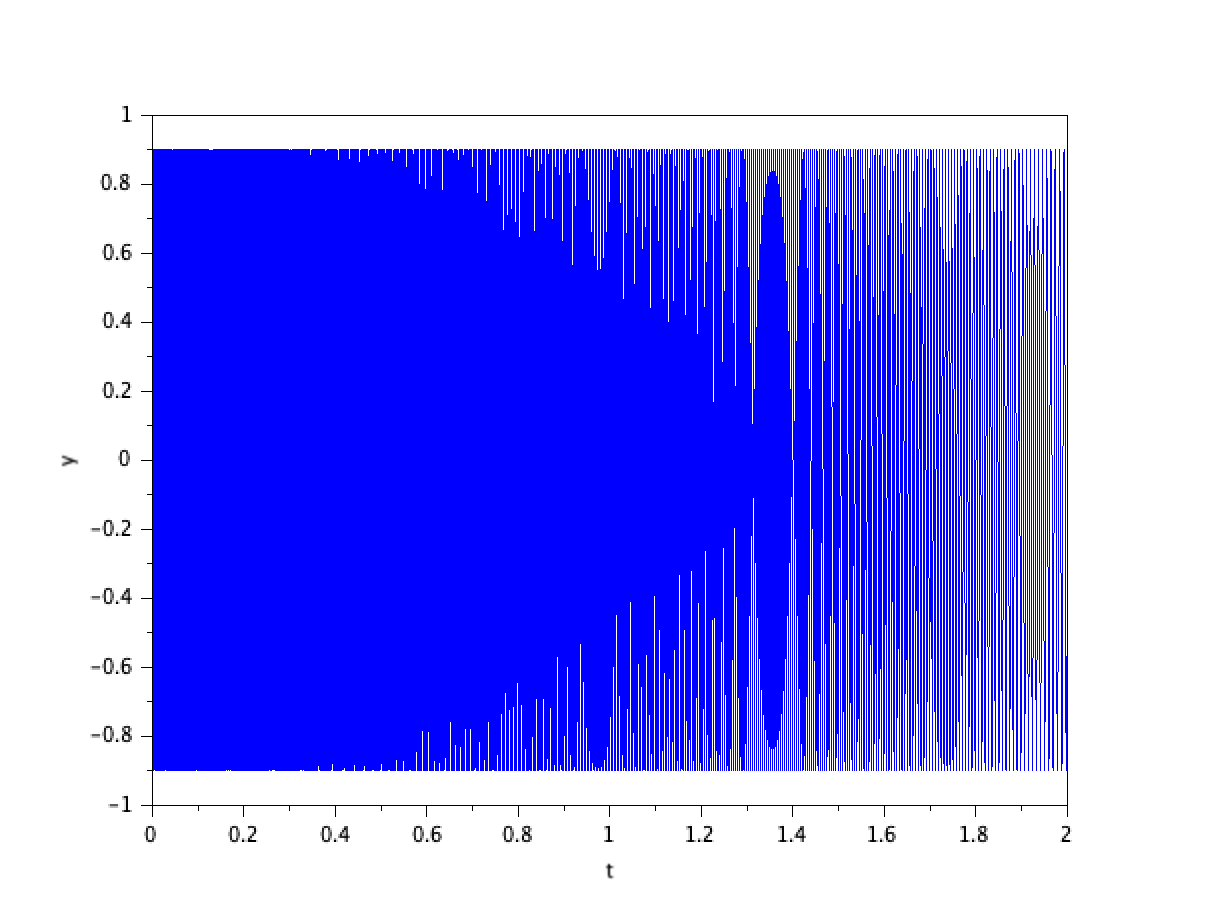
\includegraphics[width=0.8\linewidth]{picture/kadai4.png}
      \caption{演習4の出力波形}
      \label{G:kadai4}
    \end{figure}
    本実験では,周波数が$\SI{500}{\hertz} \sim \SI{300}{\hertz}$まで時間とともに低くなる音を作成した.
    図\ref{G:kadai4}からも時間が経過するごとにどんどん周波数が低くなっていることがわかる.

  \subsection{例題6}
    ここで作成したソースコードを以下のCode\ref{C:reidai6}に示す.また,作成した音をフーリエ変換したグラフ
    を図\ref{G:reidai6}に示す.
    \lstinputlisting[caption=例題6のソースコード, label=C:reidai6]{Sci_data/reidai6.sce}
    \begin{figure}[H]
      \centering
      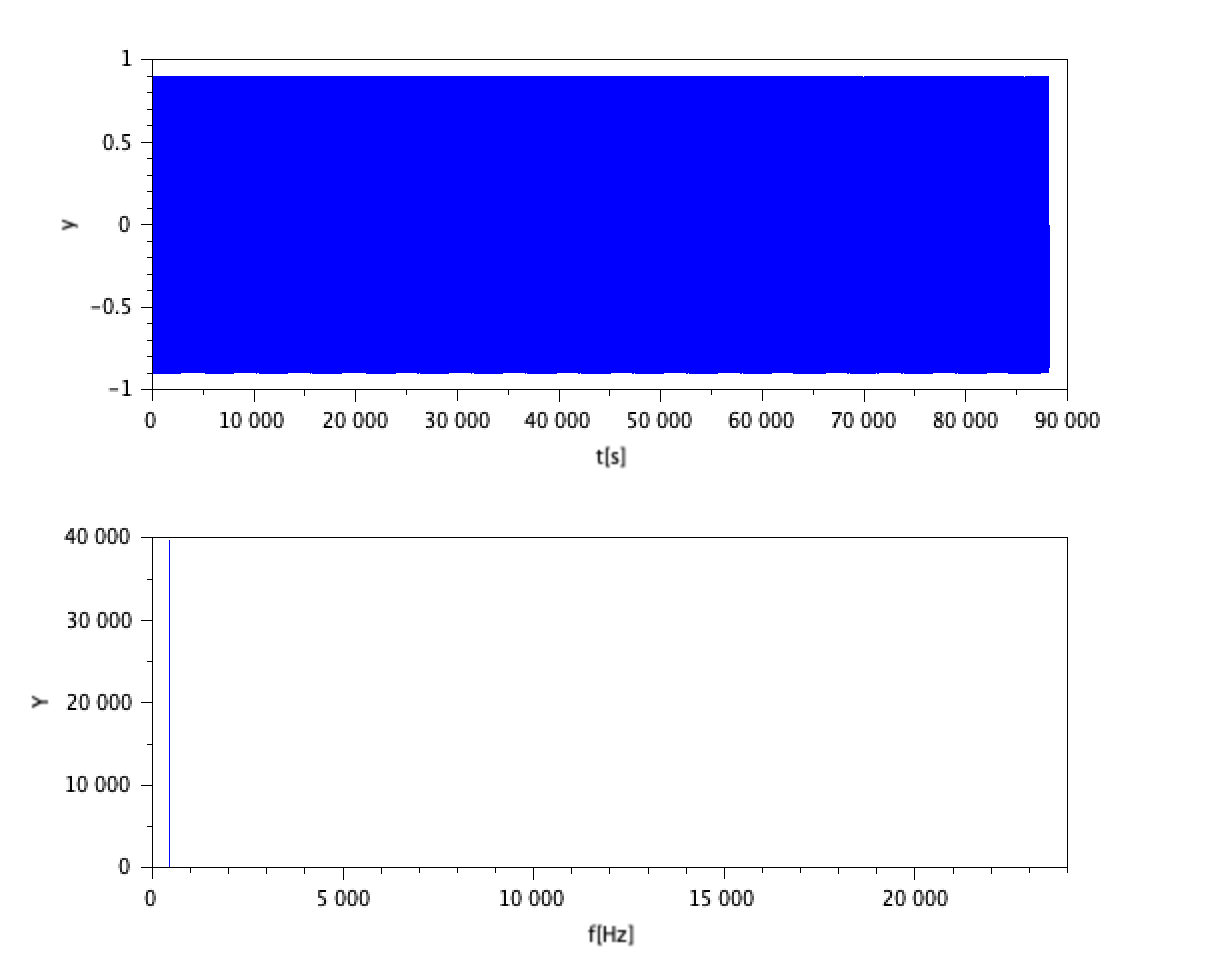
\includegraphics[width=0.8\linewidth]{picture/reidai6.png}
      \caption{例題6の出力波形}
      \label{G:reidai6}
    \end{figure}
    図\ref{G:reidai6}からわかるように,$\SI{440}{\hertz}$の波形をフーリエ変換すると,周波数軸が$\SI{440}{\hertz}$
    のところに一本だけ線がでるグラフが出力される

  \subsection{例題7}
    ここで作成したソースコードを以下のCode\ref{C:reidai7}に示す.また,作成したグラフ
    を図\ref{G:reidai7}に示す.
    \lstinputlisting[caption=例題7のソースコード, label=C:reidai7]{Sci_data/reidai7.sce}
    \begin{figure}[H]
      \centering
      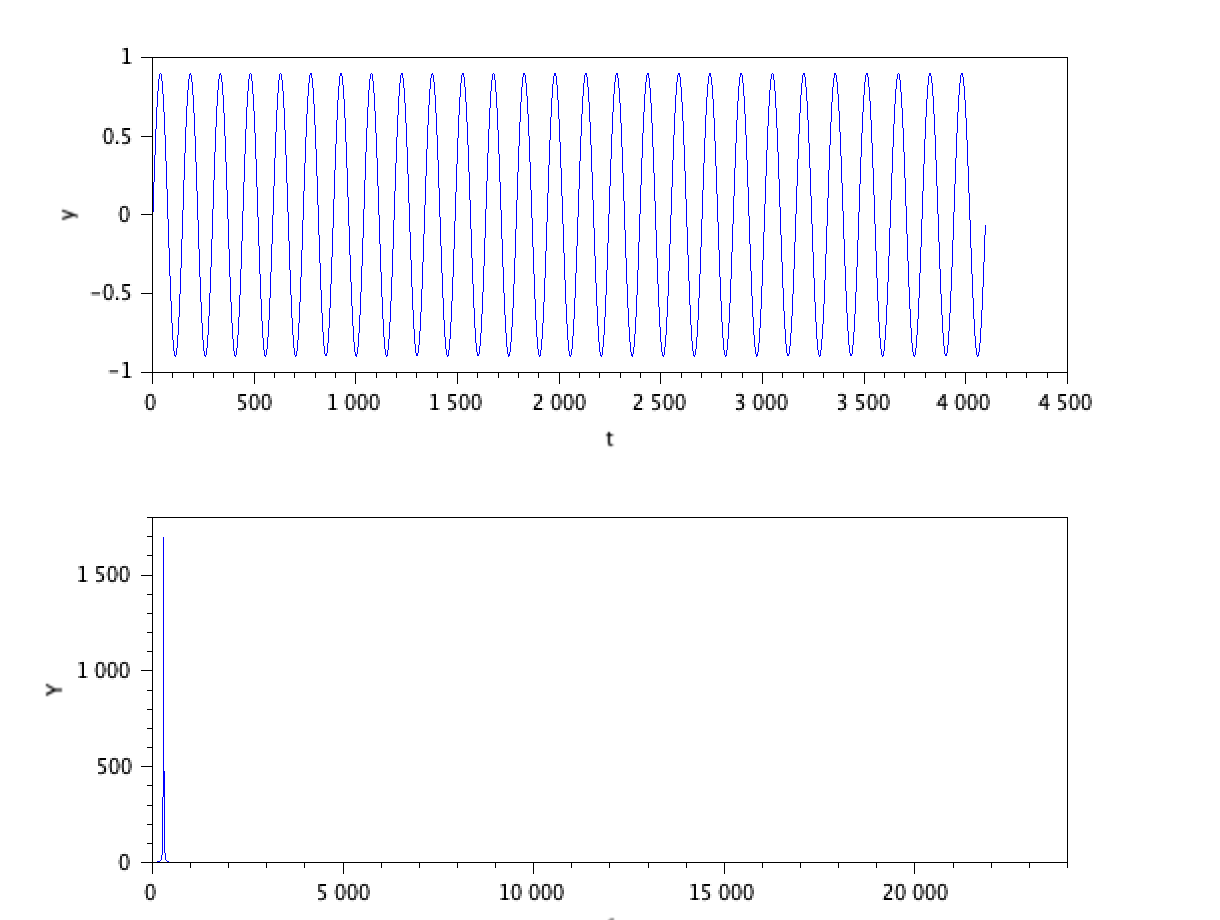
\includegraphics[width=0.8\linewidth]{picture/reidai7.png}
      \caption{例題7の出力波形}
      \label{G:reidai7}
    \end{figure}
    例題7ではこれまでの信号とは違い,非定常信号に適用できる方法でフーリエ変換を行っている.これを
    短時間フーリエ変換といい,非定常信号から取り出した一部が無限に繰り返されていると仮定してフーリエ変換を
    行っている.

  \subsection{例題8}
  ここで作成したソースコードを以下のCode\ref{C:reidai8}に示す.また,作成したグラフ
  を図\ref{G:reidai8}に示す.
  \lstinputlisting[caption=例題8のソースコード, label=C:reidai8]{Sci_data/reidai8.sce}
  \begin{figure}[H]
    \centering
    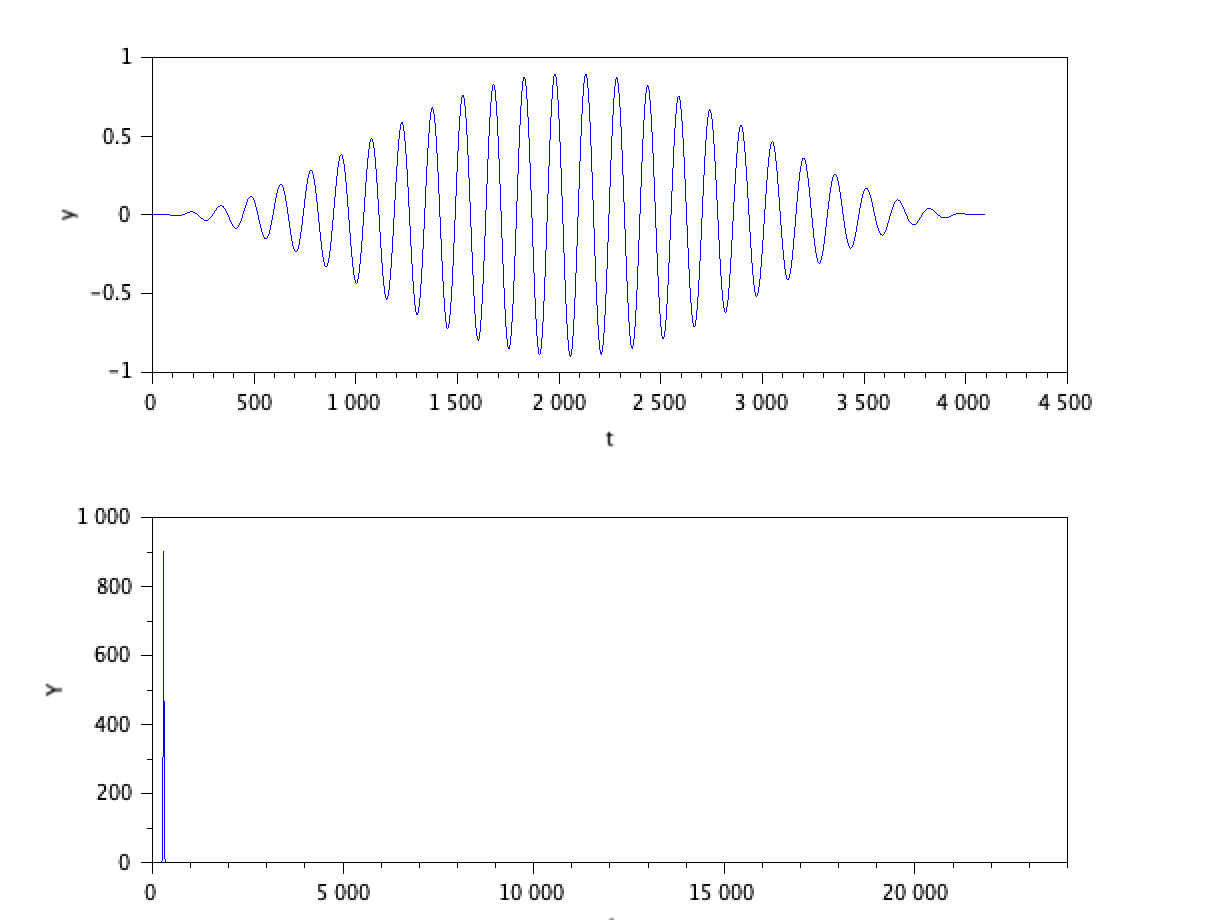
\includegraphics[width=0.8\linewidth]{picture/reidai8.png}
    \caption{例題8の出力波形}
    \label{G:reidai8}
  \end{figure}
  図\ref{G:reidai8}のフーリエ変換後のグラフより,窓関数をかけることによりそこの範囲だけ切り取ることが
  できていることがわかる.

  \subsection{演習9}
    \begin{screen}
      $h$の長さを長くして信号$sn$に畳み込むと,$fsn$はどうなるかを試せ.
    \end{screen}
    ここで作成したソースコードを以下のCode\ref{C:kadai9}に示す.また,作成したグラフ
  を図\ref{G:kadai9_3},\ref{G:kadai9_5}に示す.
  \lstinputlisting[caption=課題9のソースコード, label=C:kadai9]{Sci_data/kadai9.sce}
  \begin{figure}[H]
    \begin{tabular}{cc}
      \begin{minipage}[t]{0.48\textwidth}
        \centering
        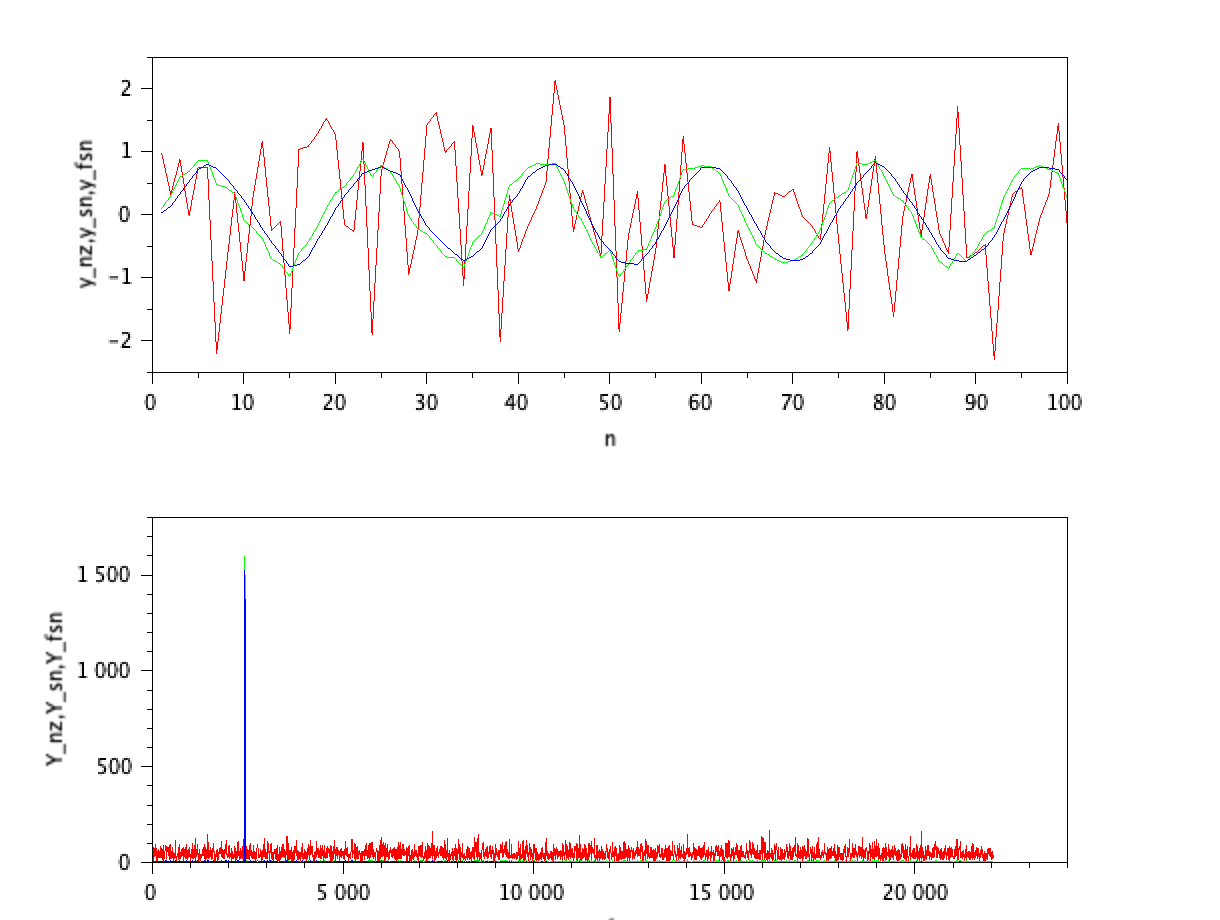
\includegraphics[clip,width=9cm]{picture/kadai9_h3.png}
        \caption{$h = 0.3333の場合$}
        \label{G:kadai9_3}
      \end{minipage} &
      \begin{minipage}[t]{0.48\textwidth}
        \centering
        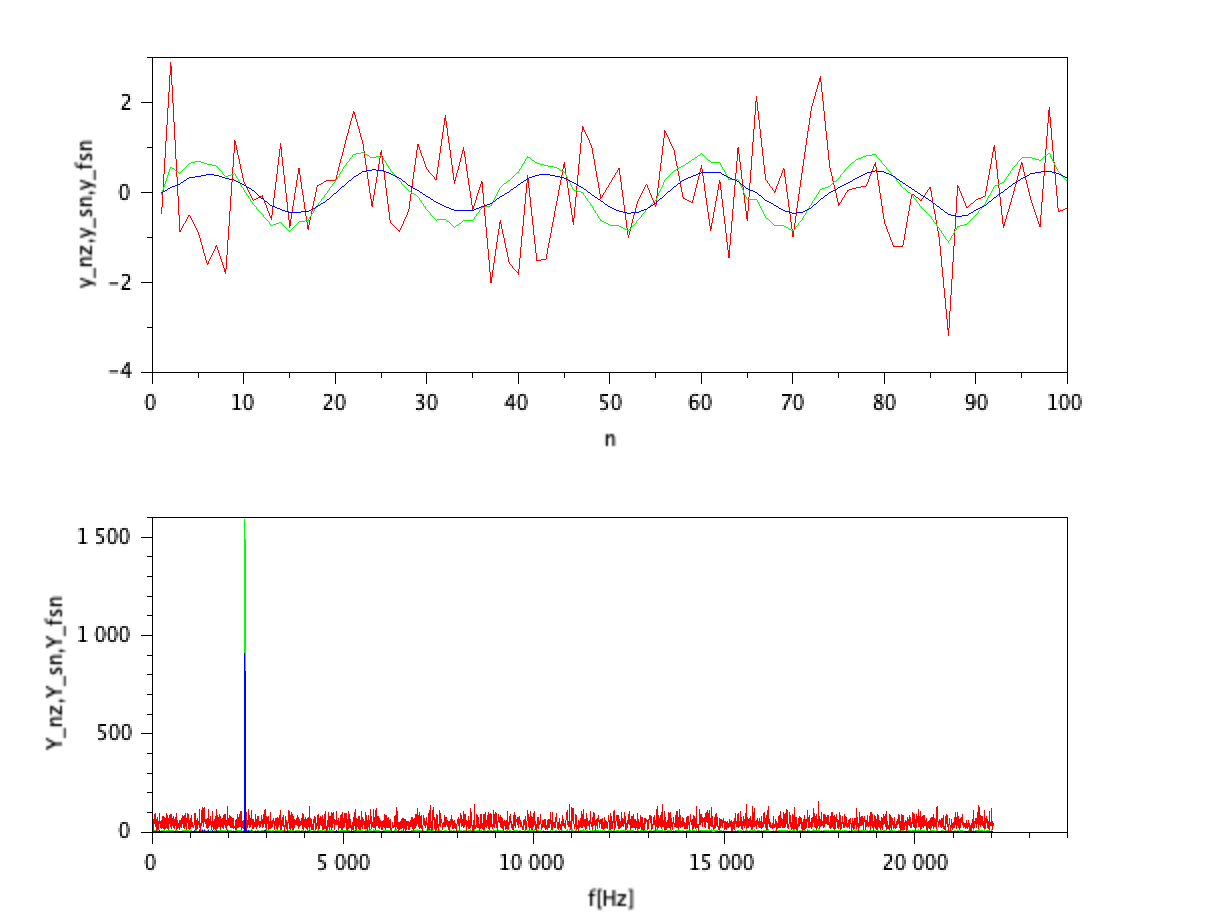
\includegraphics[clip,width=9cm]{picture/kadai9_h5.png}
        \caption{$h = 0.2$の場合}
        \label{G:kadai9_5}
      \end{minipage}
    \end{tabular}
  \end{figure}
  ここでは,$h$の値を変化させ,フィルターによる波形への影響を確認した.$h=0.33\cdots$のときと$h=0.2$のときを比べると,わずかに$h=0.33\cdots$のほうが
  sin波形がなめらかになった.その代わり,振幅が多少小さくなることがわかった.

  \subsection{演習13}
    \begin{screen}
      \textbf{wfir}を用いて,$\SI{550}{\hertz}$以下の低減だけを通過させる\textbf{LPF}を設計し,その\textbf{LPF}
      を$s_n$に適用せよ.
  \end{screen}  
  ここで作成したソースコードを以下のCode\ref{C:kadai13}に示す.また,作成したグラフ
  を図\ref{G:kadai13}に示す.
  \lstinputlisting[caption=演習13のソースコード, label=C:kadai13]{Sci_data/kadai13.sce}
  \begin{figure}[H]
    \centering
    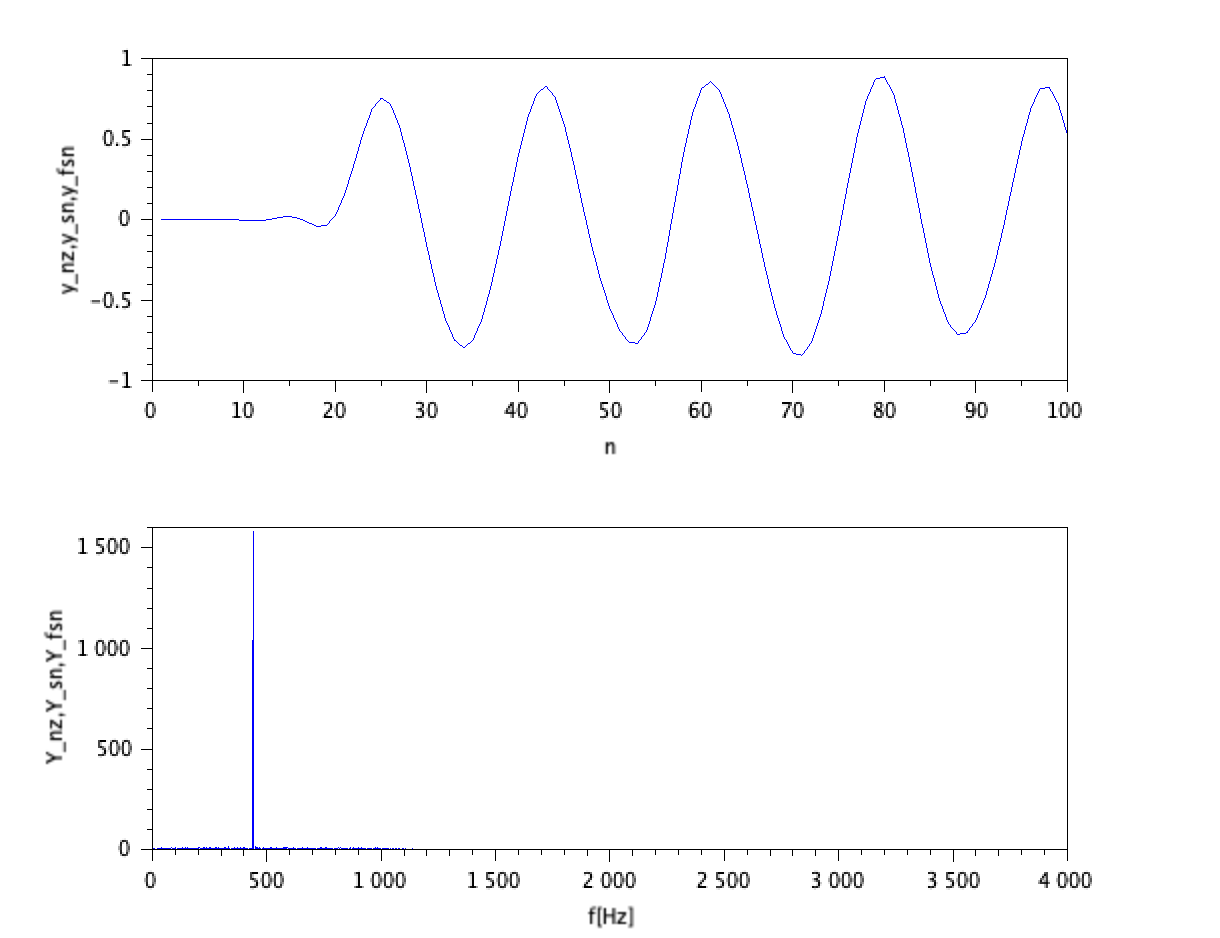
\includegraphics[width=0.8\linewidth]{picture/kadai13.png}
    \caption{演習13の出力波形}
    \label{G:kadai13}
  \end{figure}
  図\ref{G:kadai13}からもわかるように,$\SI{550}{\hertz}$以下のみが出力されており,それ以上はカットされている.
  よってローパスフィルタが正常に動作していることがわかる.

  \subsection{演習14}
    \begin{screen}
      \textbf{wfir}を用いて,ある周波数以上の広域を通過させるフィルタ(ハイパスフィルタ,\textbf{HPF})も
      設計できる.$\SI{450}{\hertz}$以上を通過させる\textbf{HPF}を設計し,その\textbf{HPF}を$s_n$に適用せよ.
    \end{screen}
    ここで作成したソースコードを以下のCode\ref{C:kadai14}に示す.また,作成したグラフ
  を図\ref{G:kadai14}に示す.
  \lstinputlisting[caption=演習14のソースコード, label=C:kadai14]{Sci_data/kadai14.sce}
  \begin{figure}[H]
    \centering
    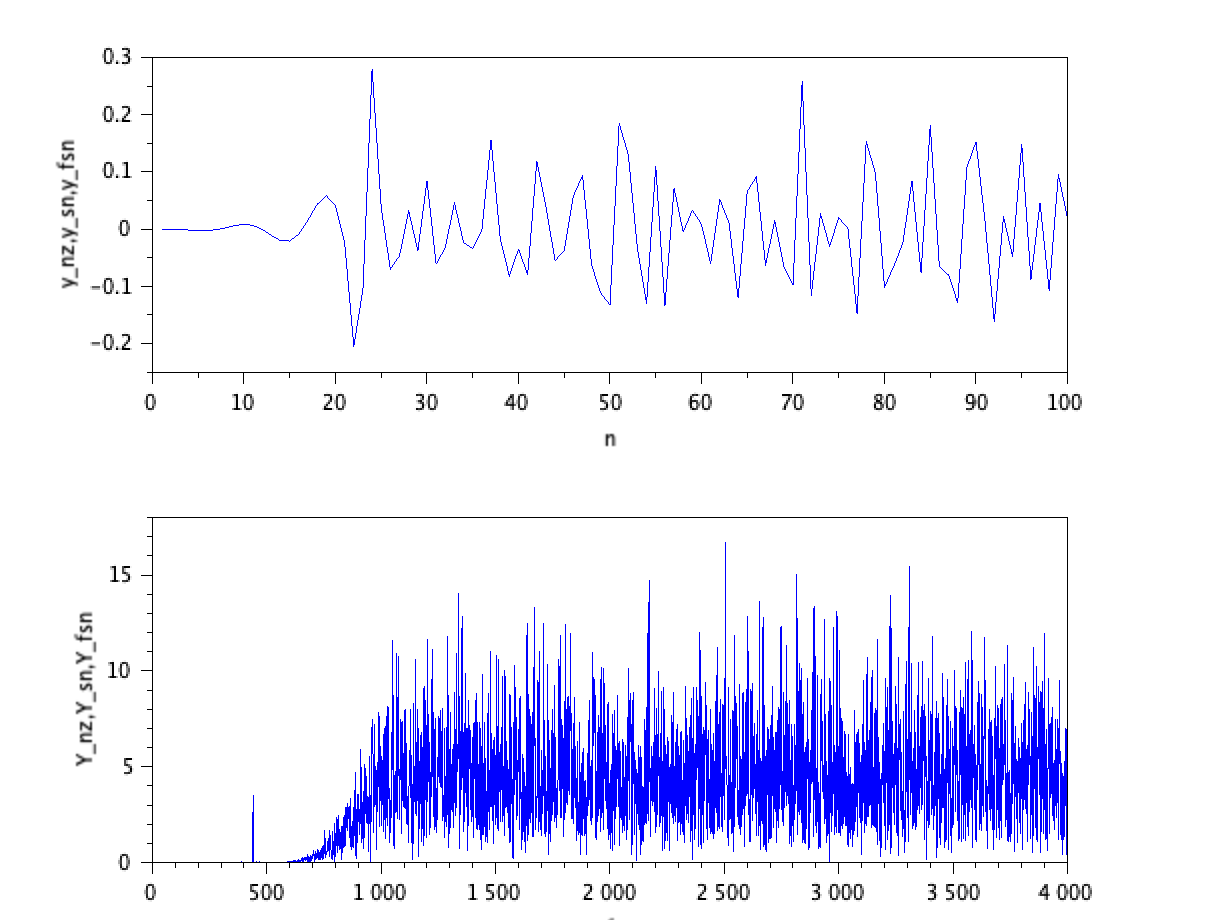
\includegraphics[width=0.8\linewidth]{picture/kadai14.png}
    \caption{演習14の出力波形}
    \label{G:kadai14}
  \end{figure}
  図\ref{G:kadai14}からもわかるように,$\SI{450}{\hertz}$以上の周波数だけが出力されていることがわかる.よってハイパスフィルタが
  正常に動作していることがわかる.

\section{考察}

\begin{thebibliography}{99}
  \bibitem{text} 野尻 紘聖: 信号処理, 制御情報システム工学実験2 実験指導書  (最終閲覧日 2021年5月25日)\\
  \bibitem{sampling} 嵯峨山 茂樹: 音声解析(1)サンプリングと量子化, 東京大学 工学部 計数工学科/物理工学科 (最終閲覧日 2021年5月25日)\\ 
  \url{https://ocw.u-tokyo.ac.jp/lecture_files/engin_01/2/notes/ja/B1-Sampling.pdf}
  \bibitem{window} ロジカルアーツ研究所: 窓関数を用いる理由 (最終閲覧日 2021年5月26日) \\ \url{https://www.logical-arts.jp/archives/124}
\end{thebibliography}


\end{document}